\documentclass{article}

\usepackage{fancyhdr}
\usepackage{extramarks}
\usepackage{amsmath}
\usepackage{amsthm}
\usepackage{amsfonts}
\usepackage{tikz}
\usepackage[plain]{algorithm}
\usepackage{algpseudocode}
\usepackage{graphicx}
\usepackage{csquotes}
\usepackage{caption}
\usepackage{subcaption}
\usepackage{hyperref}
\hypersetup{
    colorlinks=true,
    linkcolor=blue,
    filecolor=blue,
    urlcolor=blue
}

\usetikzlibrary{automata,positioning}

%
% Basic Document Settings
%

\topmargin=-0.45in
\evensidemargin=0in
\oddsidemargin=0in
\textwidth=6.5in
\textheight=9.0in
\headsep=0.25in

\linespread{1.1}

\pagestyle{fancy}
\lhead{\hmwkAuthorName}
\chead{\hmwkClass\ (\hmwkClassInstructor): \hmwkTitle}
\rhead{\firstxmark}
\lfoot{\lastxmark}
\cfoot{\thepage}

\renewcommand\headrulewidth{0.4pt}
\renewcommand\footrulewidth{0.4pt}

\setlength\parindent{0pt}

%
% Create Problem Sections
%

\newcommand{\enterProblemHeader}[1]{
    \nobreak\extramarks{}{Problem \arabic{#1} continued on next page\ldots}\nobreak{}
    \nobreak\extramarks{Problem \arabic{#1} (continued)}{Problem \arabic{#1} continued on next page\ldots}\nobreak{}
}

\newcommand{\exitProblemHeader}[1]{
    \nobreak\extramarks{Problem \arabic{#1} (continued)}{Problem \arabic{#1} continued on next page\ldots}\nobreak{}
    \stepcounter{#1}
    \nobreak\extramarks{Problem \arabic{#1}}{}\nobreak{}
}

\setcounter{secnumdepth}{0}
\newcounter{partCounter}
\newcounter{homeworkProblemCounter}
\setcounter{homeworkProblemCounter}{1}
\nobreak\extramarks{Problem \arabic{homeworkProblemCounter}}{}\nobreak{}

%
% Homework Problem Environment
%
% This environment takes an optional argument. When given, it will adjust the
% problem counter. This is useful for when the problems given for your
% assignment aren't sequential. See the last 3 problems of this template for an
% example.
%
\newenvironment{homeworkProblem}[1][-1]{
    \ifnum#1>0
        \setcounter{homeworkProblemCounter}{#1}
    \fi
    \section{Problem \arabic{homeworkProblemCounter}}
    \setcounter{partCounter}{1}
    \enterProblemHeader{homeworkProblemCounter}
}{
    \exitProblemHeader{homeworkProblemCounter}
}

%
% Homework Details
%   - Title
%   - Due date
%   - Class
%   - Section/Time
%   - Instructor
%   - Author
%

\newcommand{\hmwkTitle}{Assignment\ \#2}
\newcommand{\hmwkDueDate}{September 29, 2020}
\newcommand{\hmwkClass}{SCI 238}
\newcommand{\hmwkClassInstructor}{Dr. Michael Fich}
\newcommand{\hmwkAuthorName}{\textbf{Zach Bortoff}}

%
% Title Page
%

\title{
    \vspace{2in}
    \textmd{\textbf{\hmwkClass:\ \hmwkTitle}}\\
    \normalsize\vspace{0.1in}\small{Due\ on\ \hmwkDueDate\ at 11:59pm}\\
    \vspace{0.1in}\large{\textit{\hmwkClassInstructor}}
    \vspace{3in}
}

\author{\hmwkAuthorName}
\date{}

\renewcommand{\part}[1]{\textbf{\large Part \Alph{partCounter}}\stepcounter{partCounter}\\}

%
% Various Helper Commands
%

% Useful for algorithms
\newcommand{\alg}[1]{\textsc{\bfseries \footnotesize #1}}

% For derivatives
\newcommand{\deriv}[1]{\frac{\mathrm{d}}{\mathrm{d}x} (#1)}

% For partial derivatives
\newcommand{\pderiv}[2]{\frac{\partial}{\partial #1} (#2)}

% Integral dx
\newcommand{\dx}{\mathrm{d}x}

% Alias for the Solution section header
\newcommand{\solution}{\textbf{\large Solution}}

% Probability commands: Expectation, Variance, Covariance, Bias
\newcommand{\E}{\mathrm{E}}
\newcommand{\Var}{\mathrm{Var}}
\newcommand{\Cov}{\mathrm{Cov}}
\newcommand{\Bias}{\mathrm{Bias}}

\begin{document}

\maketitle

\pagebreak

\begin{homeworkProblem}
	Assuming that both Jupiter and the Earth have circular orbits, how large will Jupiter appear to be (i.e. what is its angular diameter?) (a) at Opposition, and (b) at Conjunction? Assume that the radius of Jupiter is \(69.9\times10^3\) km and that its orbital radius is \(5.20\) A.U. (Marks: 3)\\

    \textbf{Solution}
    
    (a) This problem can be solved by first drawing a diagram of the orbits of the Earth and Jupiter, and the angular diameter of Jupiter as seen from the Earth. \\
    
    \begin{figure}[!h]
       	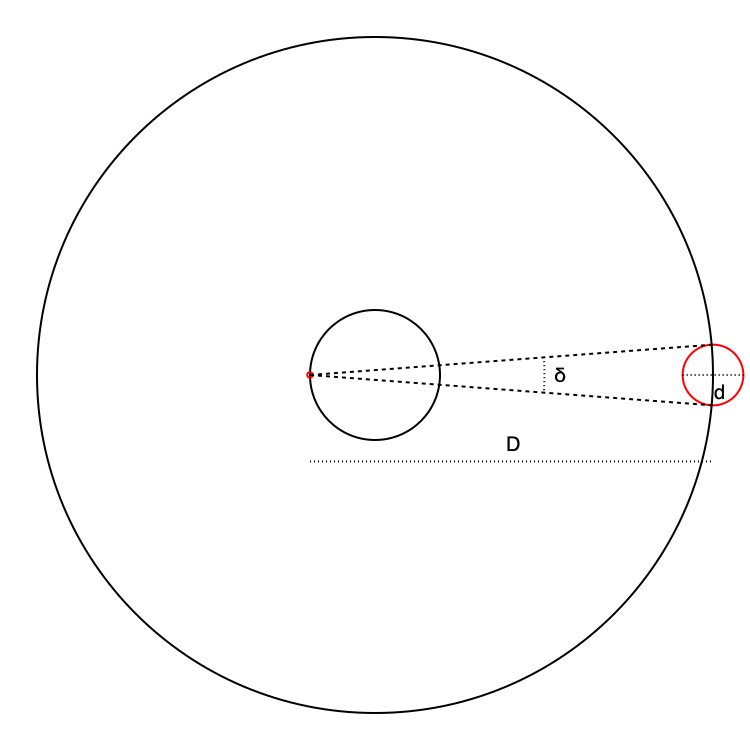
\includegraphics[width=0.5\textwidth]{OppositionDiagram.png}
        	\centering
    		\caption{Orbital Diagram of Jupiter and Earth with radii of the Earth and of Jupiter blown-up 1000 times for clarity (made diagram with Julia)}
    		\label{fig:Earth}
    	\end{figure}
    
    The variable \(D\) represents the distance between the center of the Earth and the center of Jupiter. Because the distance from the Earth to the center of the solar system is \(1\) A.U. and the distance between Jupiter and the center of the solar system is \(5.2\) A.U., it follows that \(D=1.0 + 5.2=6.2\) A.U.\\
    
    The variable \(d\) represents the diameter of Jupiter, which is \(d=2r=2(69.9 \times 10^3)\) km \(\approx0.000935\) A.U.\\
    
	Simple geometry yields:
	
	\[
		\begin{split}
			tan(\delta/2) = \frac{d/2}{D}
		\end{split}
	\]
	
	Solving for \(\delta\) yields:
	
	\[
		\begin{split}
			\delta = 2arctan(\frac{d}{2D})=2arctan(\frac{0.000935}{2(6.2)})\approx 0.000151 \space \space [rad]\approx 31.1^\circ \space \space [arcsec]
		\end{split}
	\]
	
\pagebreak

	(b) This problem can be solved in the same manner as the previous problem with one small modification. \\
    
    \begin{figure}[!h]
       	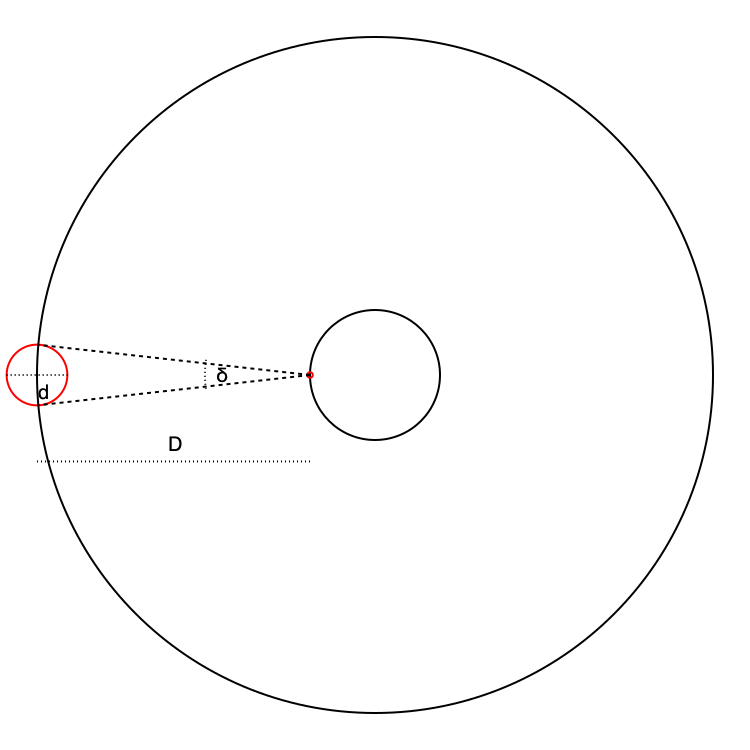
\includegraphics[width=0.5\textwidth]{ConjunctionDiagram.png}
        	\centering
    		\caption{Orbital Diagram of Jupiter and Earth with radii of the Earth and of Jupiter blown-up 1000 times for clarity (made diagram with Julia)}
    		\label{fig:Earth}
    	\end{figure}
    
    The variable \(D\) represents the distance between the center of the Earth and the center of Jupiter. Because the distance from the Earth to the center of the solar system is \(1\) A.U. and the distance between Jupiter and the center of the solar system is \(5.2\) A.U., it follows that \(D=5.2-1.0=4.2\) A.U.\\
    
    The variable \(d\) represents the diameter of Jupiter, which is \(d=2r=2(69.9 \times 10^3)\) km \(\approx0.000935\) A.U.\\
    
	Simple geometry yields:
	
	\[
		\begin{split}
			tan(\delta/2) = \frac{d/2}{D}
		\end{split}
	\]
	
	Solving for \(\delta\) yields:
	
	\[
		\begin{split}
			\delta = 2arctan(\frac{d}{2D})=2arctan(\frac{0.000935}{2(4.2)})\approx 0.000223 \space \space [rad]\approx 45.9^\circ \space \space [arcsec]
		\end{split}
	\]

\end{homeworkProblem}

\pagebreak


\begin{homeworkProblem}
 	In 1542 Copernicus was able to calculate the sizes (we now call this the semi-major axis) of the orbits for all of the planets visible without a telescope. The results of his calculations are shown in Module 2c. In 1609 Galileo measured the positions of the four largest moons of Jupiter. A portion of these observations are also shown in Module 2c. From these observations it was trivial to determine the period of the orbits of these moons. With a bit more work one can also measure the (angular) distance these moons are from Jupiter. Then in 1687 Newton published his theory of gravity. There is no evidence that anyone put these three pieces of work together to estimate the mass of Jupiter but you can do this!\\
 	
 	\textbf{Determine the mass of Jupiter} assuming (1) the semi-major axis of Jupiter's orbit is \(5.20\) A.U.; (2) the period of Ganymede's (the largest moon of Jupiter) orbit is 170 hours; (3) when Jupiter is at opposition Ganymede reaches a maximum of 5.9 arcminutes from Jupiter; (4) Ganymede's orbit is a circle. (Marks: 5)\\
 	
 	\textbf{Solution}

\end{homeworkProblem}

\pagebreak

\begin{homeworkProblem}
 	The spectrum of a star is recorded (i.e. observed). The wavelength of the "Balmer alpha" spectral line of hydrogen is measured to be at \(655.9\) nanometers (nm). If the "rest wavelength" of this spectral line is \(656.3\) nm then \textbf{what is the radial velocity of this start}? \textit{Think carefully about "significant figures" in this question. It's a bit tricky. Full marks requires exactly the correct number of significant figures in the final answer...} (Marks: 3)\\
 	
 	\textbf{Solution}

\end{homeworkProblem}
\pagebreak

\end{document}
